\documentclass[fleqn,10pt,table]{wlscirep}
\usepackage{graphicx}
\usepackage{subcaption}
\usepackage{xcolor}

\newcommand{\attn}[1]{\colorbox{red}{#1}}
\newcommand{\todo}[1]{\colorbox{yellow}{#1}}

\title{Supplemental Materials.}

\begin{document}

\begin{figure}[ht]
\centering
\begin{subfigure}{0.30\textwidth}
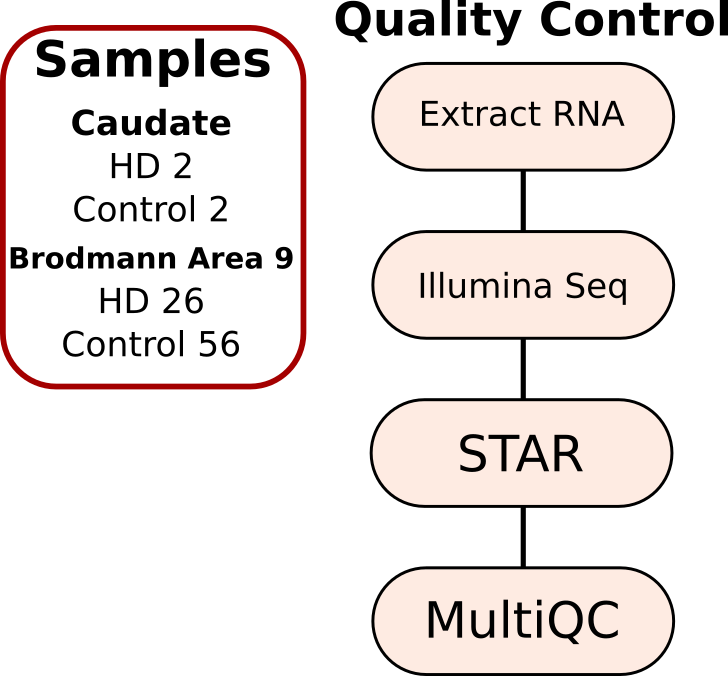
\includegraphics[width=.8\linewidth]{quality_control.png}
\caption{1a}
\label{fig:sfig1a}
\end{subfigure}
\begin{subfigure}{0.30\textwidth}
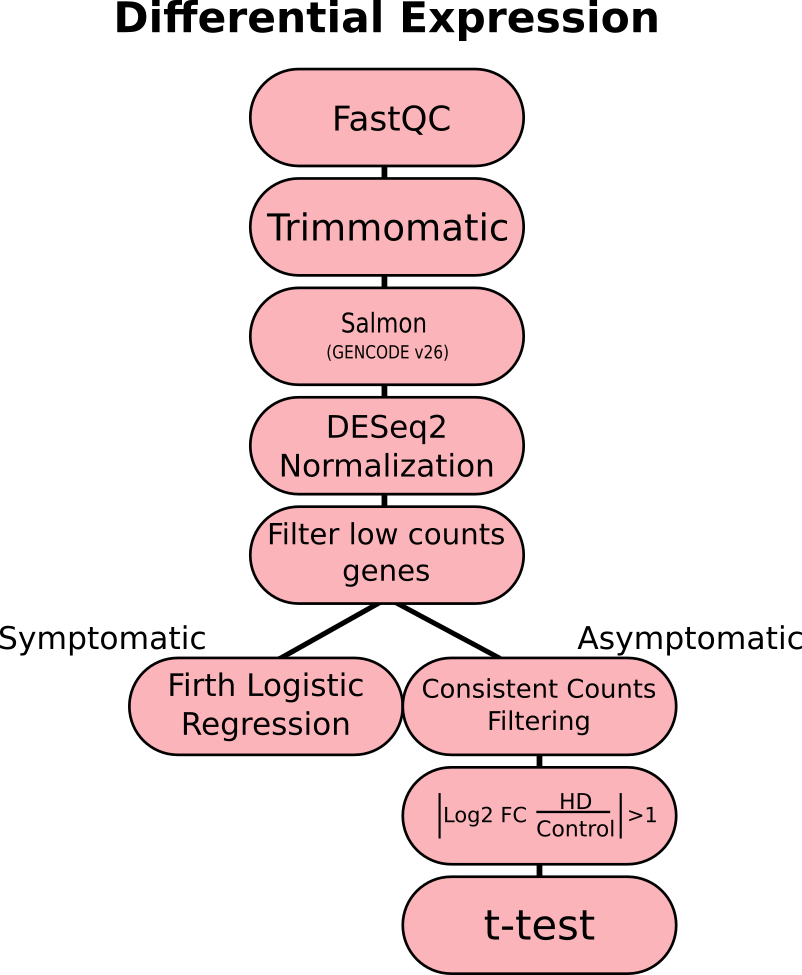
\includegraphics[width=.8\linewidth]{differential_expression.png}
\caption{1a}
\label{fig:sfig1b}
\end{subfigure}
\begin{subfigure}{0.30\textwidth}
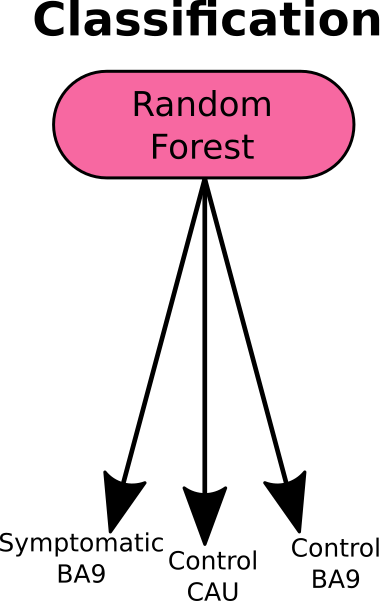
\includegraphics[width=.6\linewidth]{classification.png}
\caption{1a}
\label{fig:sfig1c}
\end{subfigure}

% Figure 1: goal of study
%\caption{sub figure A RNAseq pipeline -> Salmon + sub figure B filtering with gene numbers + sub fix C %random forest method + sub fig D all different comparisons}
%D: asymp BA9 v asymp CAP/asymp BA9 v C BA9/asymp HD CAP v C CAP
%D: symp HD BA9 v C BA9/ GTEx C BA9 v C CAP
% Outline 
\end{figure}

\end{document}